\documentclass{hdureport}

\usepackage{newunicodechar}
\newunicodechar{ε}{\ensuremath{\varepsilon}}

\course{编译原理课程实践}

\name{梅瑞贤}
\instructor{黄孝喜}
\college{计算机学院}
\major{计算机科学与技术}
\stuid{21052021}
% \authorclass{21052317}
\expname{编译理论相关算法实现}
% \date{2022}{2}{Feb}
\date{\today}
% \lab{一教115}
% \documentclass[utf8]{ctexart}
\begin{document}

\makecover

\setcounter{secnumdepth}{3}
\setcounter{tocdepth}{3}

\tableofcontents

\newpage

\section{词法分析器相关}

\subsection{实验目的}
掌握从正则表达式构造NFA的算法,掌握从NFA构造DFA的算法,掌握DFA最小化算法。
\subsection{实验内容}
编写程序,从只含有星闭包、连接和或运算的正则表达式构造NFA,并将NFA转换为DFA,最后对DFA进行最小化处理。
\subsection{设计方案与算法描述}

方案设计如下:
\begin{itemize}
    \item{将输入的正则式转化为后缀表达式,并构后缀树}
    \item{使用Tompson或者Glushkov算法将后缀树转化为NFA}
    \item{使用子集构造法将NFA转化为DFA}
    \item{使用Hopcroft算法对DFA进行最小化处理}
    \item{使用dot语言输出DFA的图形化表示}
\end{itemize}

\quad \\ 

Tompson算法:

根据语法树构造NFA,对于每个节点,如果是连接符,那么将左右子树的开始节点和结束节点分别连接起来,如果是或运算符,那么将左右子树的开始节点和结束节点分别连接到一个新的节点,如果是闭包运算符,那么将左子树的开始节点和结束节点分别连接到一个新的节点,然后将新的节点和自身连接起来,最后将新的节点和结束节点连接起来。

\quad \\ 

Glushkov算法:

根据语法树构造NFA,对于每个节点,维护开始集合、结束集合、关系集合和一个可空标志

构造NFA的过程中,对于每个节点,需要维护以下信息
\begin{itemize}
    \item 开始集合:表示从该节点开始的所有可能的输入符号集合
    \item 结束集合:表示从该节点结束的所有可能的输入符号集合
    \item 关系集合:表示一个相邻的节点对
    \item 可空标志:表示该节点是否可以为空(即可以匹配空字符串)
\end{itemize}

对于不同的节点每种集合和标志的转移如下:
\begin{itemize}
    \item 对于连接符,将左子树的开始集合和结束集合分别连接到右子树的开始集合和结束集合,如果左子树可空,那么将左子树的结束集合连接到右子树的开始集合
    \item 对于或运算符,将左子树的开始集合和结束集合分别连接到一个新的节点,将右子树的开始集合和结束集合分别连接到一个新的节点,然后将新的节点和自身连接起来,最后将新的节点和结束节点连接起来
    \item 对于闭包运算符,将左子树的开始集合和结束集合分别连接到一个新的节点,然后将新的节点和自身连接起来,最后将新的节点和结束节点连接起来
    \item 对于字符节点,将开始集合和结束集合分别连接到一个新的节点,然后将新的节点和结束节点连接起来
    \item 对于空节点,将开始集合和结束集合分别连接到一个新的节点,然后将新的节点和结束节点连接起来
\end{itemize}

最后根据根节点的关系集合构造NFA,每个关系集合中的元素表示一个转换关系,其中第一个元素表示起始节点,第二个元素表示结束节点

根据根节点的开始集合和结束集合以及可空标志构造NFA的开始节点和结束节点

\quad \\

子集构造法:

使用epsilon闭包求出NFA的开始节点的epsilon闭包,作为DFA的开始节点

然后对于DFA的每个节点,对于每个输入符号,求出NFA中该节点的epsilon闭包经过该输入符号的转移,作为DFA中该节点经过该输入符号的转移

\quad \\

Hopcroft算法:

Hopcroft算法的核心思想是将DFA中的状态划分为等价类,然后将等价类作为新的状态,构造新的DFA

Hopcroft算法的过程如下:

\begin{itemize}
    \item{将DFA中的状态划分为两个等价类,一个是终态,一个是非终态}
    \item{对于每个等价类,对于每个输入符号,求出该等价类经过该输入符号的转移,如果该等价类经过该输入符号的转移后的状态不在该等价类中,那么将该等价类划分为两个等价类,一个是该等价类经过该输入符号的转移后的状态,一个是该等价类减去该等价类经过该输入符号的转移后的状态}
    \item{重复上述过程,直到没有等价类发生变化}
    \item {将等价类作为新的状态,构造新的DFA}
    \item {将新的DFA中的状态重新编号}
    \item {将新的DFA中的终态设置为原来的终态}
    \item {将新的DFA中的开始态设置为原来的开始态}
    \item {将新的DFA中的状态按照编号排序}
\end{itemize}

\newpage

\subsection{测试结果}

\noindent\textbf{TestCase\quad 1:} 

\noindent\textsf{input:}
\lstinputlisting{dfa_test/1.in}
\noindent\textsf{output:}
\lstinputlisting{dfa_test/1.dot}
\noindent\textsf{visual:}
\begin{figure}[H]
    \centering
    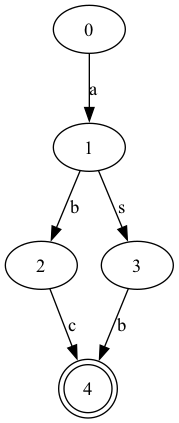
\includegraphics[width=0.3\textwidth]{dfa_test/1.png}
    \caption{Test 1}
\end{figure}

\newpage

\noindent\textbf{TestCase\quad 2:} 

\noindent\textsf{input:}
\lstinputlisting{dfa_test/2.in}
\noindent\textsf{output:}
\lstinputlisting{dfa_test/2.dot}
\newpage
\noindent\textsf{visual:}
\begin{figure}[H]
    \centering
    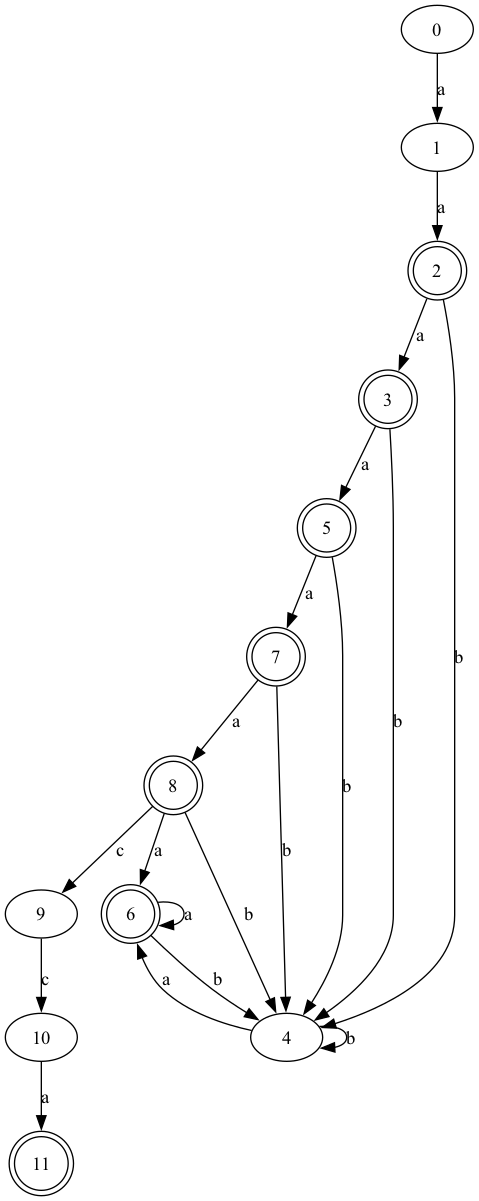
\includegraphics[width=0.5\textwidth]{dfa_test/2.png}
    \caption{Test 2}
\end{figure}

\newpage

\noindent\textbf{TestCase\quad 3:} 

\noindent\textsf{input:}
\lstinputlisting{dfa_test/3.in}
\noindent\textsf{output:}
\lstinputlisting{dfa_test/3.dot}
\newpage
\noindent\textsf{visual:}
\begin{figure}[H]
    \centering
    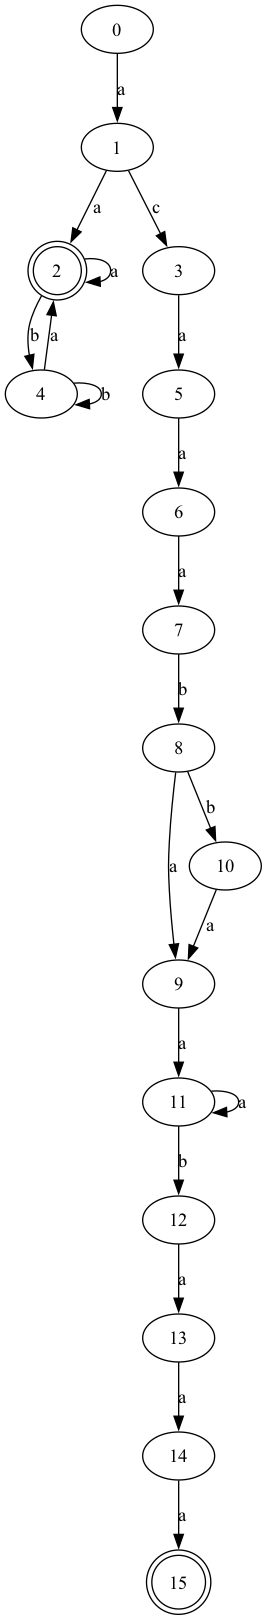
\includegraphics[width=0.21\textwidth]{dfa_test/3.png}
    \caption{Test 3}
\end{figure}

\newpage

\noindent\textbf{TestCase\quad 4:} 

\noindent\textsf{input:}
\lstinputlisting{dfa_test/4.in}
\noindent\textsf{output:}
\lstinputlisting{dfa_test/4.dot}
\newpage
\noindent\textsf{visual:}
\begin{figure}[H]
    \centering
    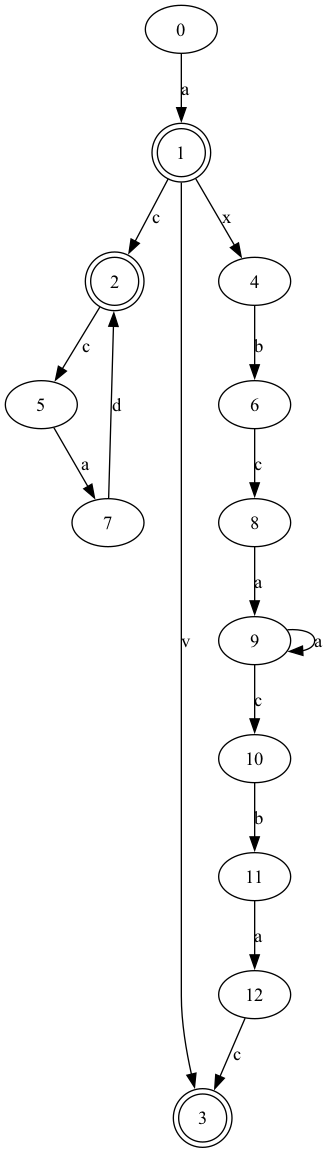
\includegraphics[width=0.35\textwidth]{dfa_test/4.png}
    \caption{Test 4}
\end{figure}

\newpage
\noindent\textbf{TestCase\quad 5:} 

\noindent\textsf{input:}
\lstinputlisting{dfa_test/5.in}
\noindent\textsf{output:}
\lstinputlisting{dfa_test/5.dot}
\noindent\textsf{visual:}
\begin{figure}[H]
    \centering
    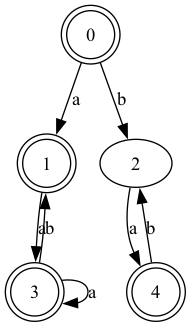
\includegraphics[width=0.3\textwidth]{dfa_test/5.png}
    \caption{Test 5}
\end{figure}

\newpage

\subsection{源代码}

\lstinputlisting[language=C++]{../DFA.cpp}

\newpage

\section{LL1文法相关}


\subsection{实验目的}
掌握从LL1文法提取公共因子,消除左递归的算法,掌握LL1文法的FIRST集和FOLLOW集的求法,掌握LL1文法的预测分析表的构造算法。

\subsection{实验内容}
编写程序,输入上下文无关文法,如果可以化简为LL1文法则输出提取公共左因子后的文法,消除左递归后的文法,FIRST集,FOLLOW集,预测分析表,否则报错。

\subsection{设计方案与算法描述}
方案设计如下:
\begin{itemize}
    \item {使用暴力进行字符串切割和匹配,将输入的文法转化为token序列}
    \item {使用trie树和dfs提取文法的左公共因子}
    \item {对提取完左公共因子的文法消去左递归}
    \item {根据定义求出FIRST集、FOLLOW集、预测分析表}
    \item {根据预测分析表进行语法分析}
\end{itemize}

\quad \\
根据trie树提取左公共因子:

经过观察,把文法全部插入到trie树中,然后对于每个节点,如果该节点的子节点数大于1,那么就将该节点的子节点的公共前缀作为公共因子,然后将该节点的子节点的公共前缀作为新的节点,将该节点的子节点的公共前缀作为新的子节点插入到新的节点中,然后将该节点的子节点的公共前缀从该节点的子节点中删除,最后将该节点的子节点的公共前缀作为新的节点的子节点。

\quad \\

消除左递归:

上课详细讲过,不多赘述

\quad \\

求FIRST等集合:

根据定义求出FIRST集、FOLLOW集、预测分析表

\newpage

\subsection{测试结果}

\noindent\textbf{TestCase\quad 1:} 

\noindent\textsf{input:}

\lstinputlisting{./ll1_test/1.in}

\noindent\textsf{output:}

\lstinputlisting{./ll1_test/1.out}

\noindent\textsf{graph:}

\begin{table}[!ht]
    \centering
    \resizebox{\textwidth}{!}{
        \begin{tabular}{|l|l|l|l|l|l|l|l|l|l|}
        \hline
            ~ & \$ & ε & + & - & * & / & ( & ) & i \\ \hline
            E & ~ & ~ & ~ & ~ & ~ & ~ & E -> T tmp0 & ~ & E -> T tmp0 \\ \hline
            T & ~ & ~ & ~ & ~ & ~ & ~ & T -> F tmp1 & ~ & T -> F tmp1 \\ \hline
            F & ~ & ~ & ~ & ~ & ~ & ~ & F -> ( E ) & ~ & F -> i \\ \hline
            tmp0 & tmp0 -> ε & ~ & tmp0 -> + T tmp0 & tmp0 -> - T tmp0 & ~ & ~ & ~ & tmp0 -> ε & ~ \\ \hline
            tmp1 & tmp1 -> ε & ~ & tmp1 -> ε & tmp1 -> ε & tmp1 -> * F tmp1 & tmp1 -> / F tmp1 & ~ & tmp1 -> ε & ~ \\ \hline
        \end{tabular}
    }
\end{table}
\newpage


\noindent\textbf{TestCase\quad 2:} 

\noindent\textsf{input:}

\lstinputlisting{./ll1_test/2.in}

\noindent\textsf{output:}

\lstinputlisting{./ll1_test/2.out}

% \noindent\textsf{graph:}

% \input{./ll1_test/2.tex}
\newpage

\newcommand{\testCase}[2]{%
    \noindent\textbf{TestCase\quad #1:} 

    \noindent\textsf{input:}

    \lstinputlisting{./ll1_test/#1.in}

    \noindent\textsf{output:}

    \lstinputlisting{./ll1_test/#1.out}
    \newpage

    % if #2 {
    \noindent\textsf{graph:}

    \input{./ll1_test/#1.tex}
    % }
    \newpage
}

\foreach \i in {3,...,12} {
    \testCase{\i}{true}
}
% \testCase{3}{true}
% \testCase{4}{true}
% \testCase{5}{true}
% \testCase{6}{true}
% \testCase{7}{true}


\subsection{源代码}
\lstinputlisting[language=C++]{../LL1.cpp}

\end{document}
\newpage


